\documentclass[a4paper,12pt]{article}
\usepackage{graphicx}
\graphicspath{ {./images/} }
\usepackage{wrapfig}

\usepackage{fontspec}
\setmainfont{Exo 2}[%
    Path            =   fonts/,
    Extension       =   .otf,
    UprightFont     =   *-Regular,
    ItalicFont      =   *-Italic,
    BoldFont        =   *-Bold,
    BoldItalicFont  =   *-BoldItalic,
    FontFace        =   {black}{n}{*-Black},
    FontFace        =   {black}{it}{*-BlackItalic},
]


\usepackage[utf8]{inputenc}
\usepackage[english]{babel}

\usepackage{hyperref}
\hypersetup{
  colorlinks=true,
  linkcolor=blue,
  filecolor=magenta,      
  urlcolor=cyan,
  pdftitle={RH Soil Sediment Sampling},
  bookmarks=true,
  %pdfpagemode=FullScreen,
}
%\urlstyle{same}

\title{A Surface Soil Sediment Profile for Dar es Salaam, Tanzania}
\author{Humanitarian OpenStreetMap Team and JBA Consulting}
\usepackage[nodayofweek,level]{datetime}
\newdate{date}{28}{02}{2019}
\date{\displaydate{date}}

\newcommand*{\vcenteredhbox}[1]{\begingroup
\setbox0=\hbox{#1}\parbox{\wd0}{\box0}\endgroup}

\begin{document}
\vbox{
  \centering
  Prepared for:
  \vcenteredhbox{
\includegraphics[width=2cm]{UK-aid_logo.png}}
  and  
  \vcenteredhbox{
\includegraphics[width=6cm]{World_Bank_Group_logo.png}}
  \
  \

  

  by:
  \vcenteredhbox{
\includegraphics[width=4cm]{HOT_logo_with_text.png}}
  and
  \vcenteredhbox{
\includegraphics[width=2cm]{JBA_logo.png}}
  \maketitle
}

\newpage
\section{Executive Summary}
\label{executivesummary}
With the support of the World Bank in Tanzania, Ramani Huria (RH) and JBA Consulting partnered in October 2018 to develop a surface soil sediment dataset for the greater Dar es Salaam region of Tanzania.  This was intended to support a geomorphological assessment taking into account soil sediment characteristics for erosion and flood risk studies. 

A national-level soil profile had existed for Tanzania prior to this effort, but contained only a single sample from Dar es Salaam. This was not sufficient to analyse erosion potential across the city. The JBA team in consultation with Ramani Huria decided to use a 2km grid, which resulted in 731 sampling points being pre-established throughout the city.

A team of 10 field mappers and 4 office technicians---all Tanzanian youth participants in the Ramani Huria project---were trained in sample collection and analysis (sieving). A total of 643 points were sampled and sieved; 88 sites were inaccessible for one or another reason.

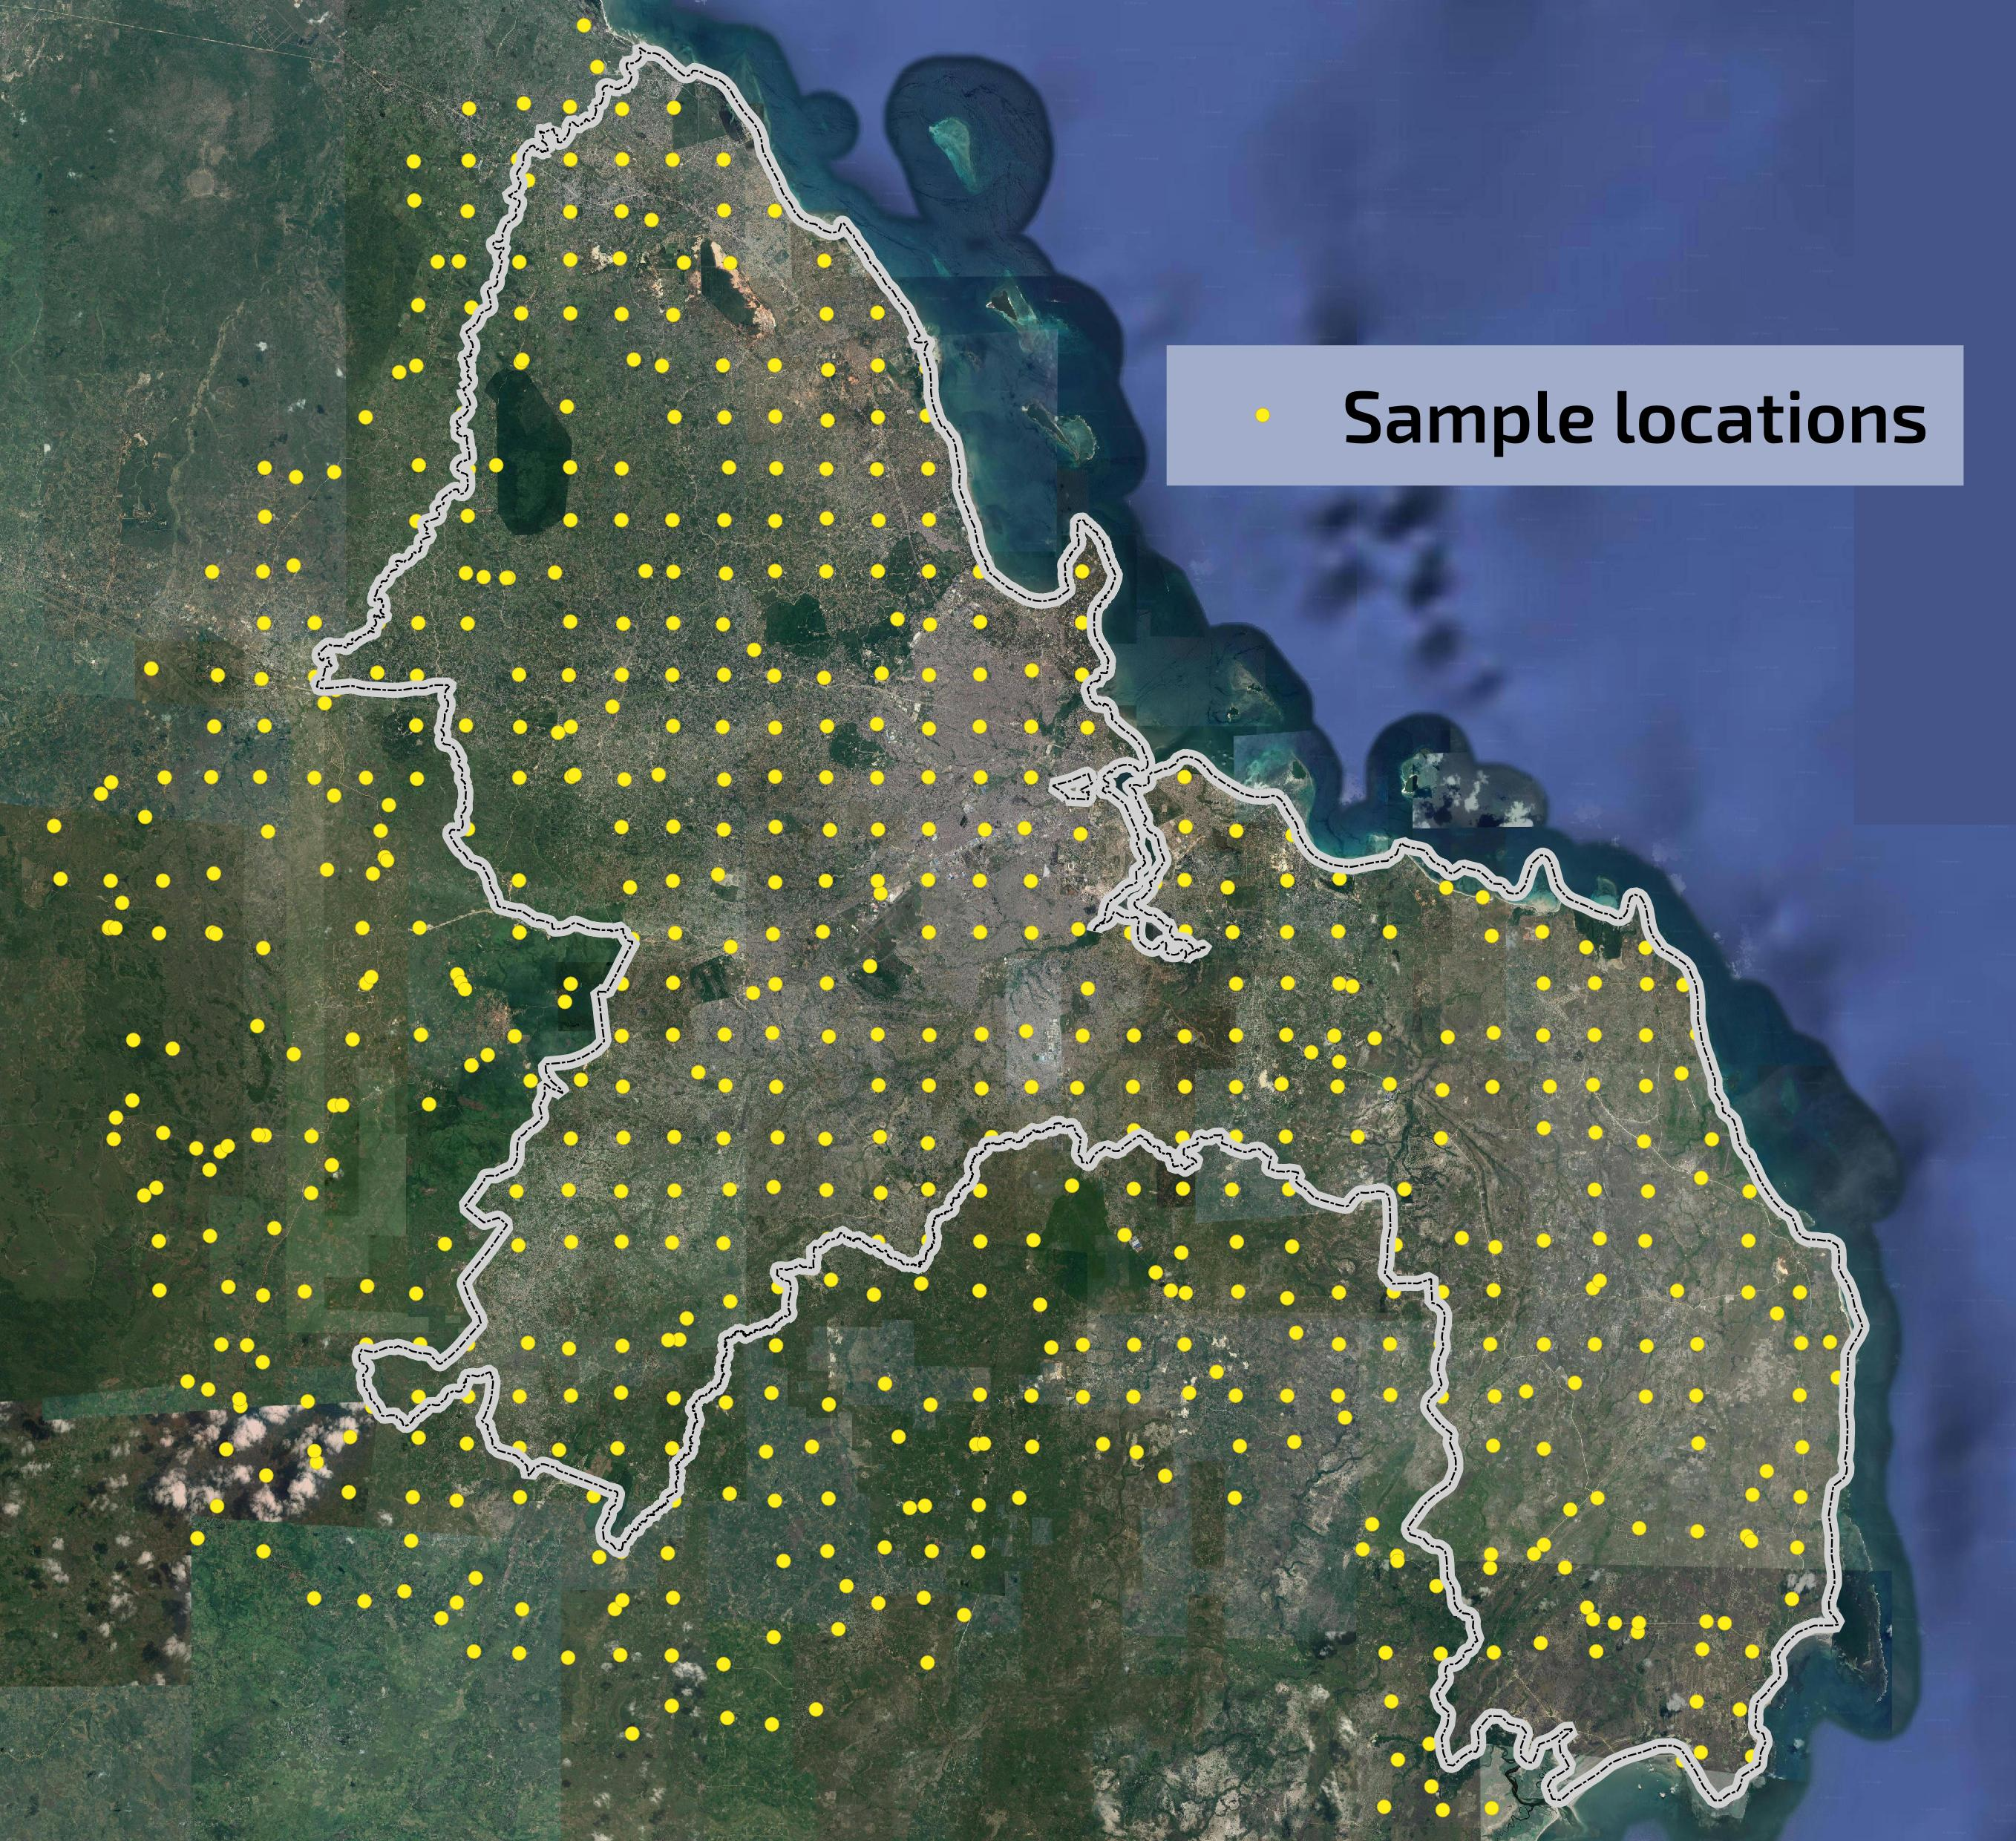
\includegraphics[width=0.8\textwidth]{sample_locations.jpg}

The 643 samples were analyzed by sieving each to separate the sediment by particle size and weighing the resulting fractions. The resulting dataset, a geo-referenced set of soil sediment profiles, is published and available as open data.


\newpage
\section{Methodology}
\label{methodology}

\subsection{Field Sample Collection}
\label{fieldsamplecollection}
Two samples of 0.5kg of sediment were collected in the field at---or if inaccessible, within 500m of---each of the pre-established sites. One sample was collected near the surface (after discarding 3cm of overlay), and the other at a depth between 7 and 15cm.

A set of data was recorded at each site using OpenDataKit's Android application ODK Collect. The team developed a form specific to this exercise. It included:
\begin{itemize}
  \item A GPS point
  \item Selection from a list of the Region, District, Ward, and Subward
  \item The ID number of the sample site (from the numbering of the 2km grid)
  \item A photograph before, during, and after the collection
  \item Information on accessibility
  \item A note if the weather was wet or dry
  \item Characteristics of the site (loose or consolidated sediment, low, medium, or high vegetation cover, rural or urban setting)
  \item A photo facing outward from the site in each cardinal direction
\end{itemize}

A copy of the field data collection form design in its original spreadsheet format is included in annex A (forms).

The team used a Kobo Toolbox instance as the back end (server) for the data collection. It was hosted on Digital Ocean, and set up using the procedure detailed \href{https://github.com/ivangayton/setup-scripts-various}{here}\footnote{\url {https://github.com/ivangayton/setup-scripts-various}. See the Readme and the file kobotoolbox\_secured\_server\_docker\_install}. The survey form was uploaded to this server, allowing all team members to download the black survey form, fill it out offline on their phones, and upload data back to the server. 

\newpage
\subsubsection{Materials}
Each field sampling team of two people carried the following equipemnt:
\begin{wrapfigure}{r}{0.25\textwidth}
  \centering
  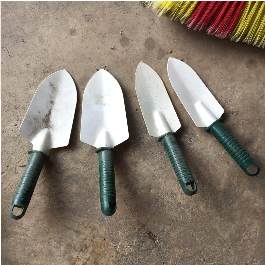
\includegraphics[width=0.25\textwidth]{trowels.png}
\end{wrapfigure}

\begin{itemize}
  \item Trowel or small shovel
  \item Plastic ``ziploc'' bags with ~1kg capacity
  \item Android phone pre-loaded with ODK Collect
  \item A separate maps and navigation application, maps.me, pre-loaded with the locations to be visited (the 2km grid)
  \item First aid kit
  \item Marker pens
  \item Permission letter for the sampling activity from the municipal authorities
  \item Tape measure
\end{itemize}

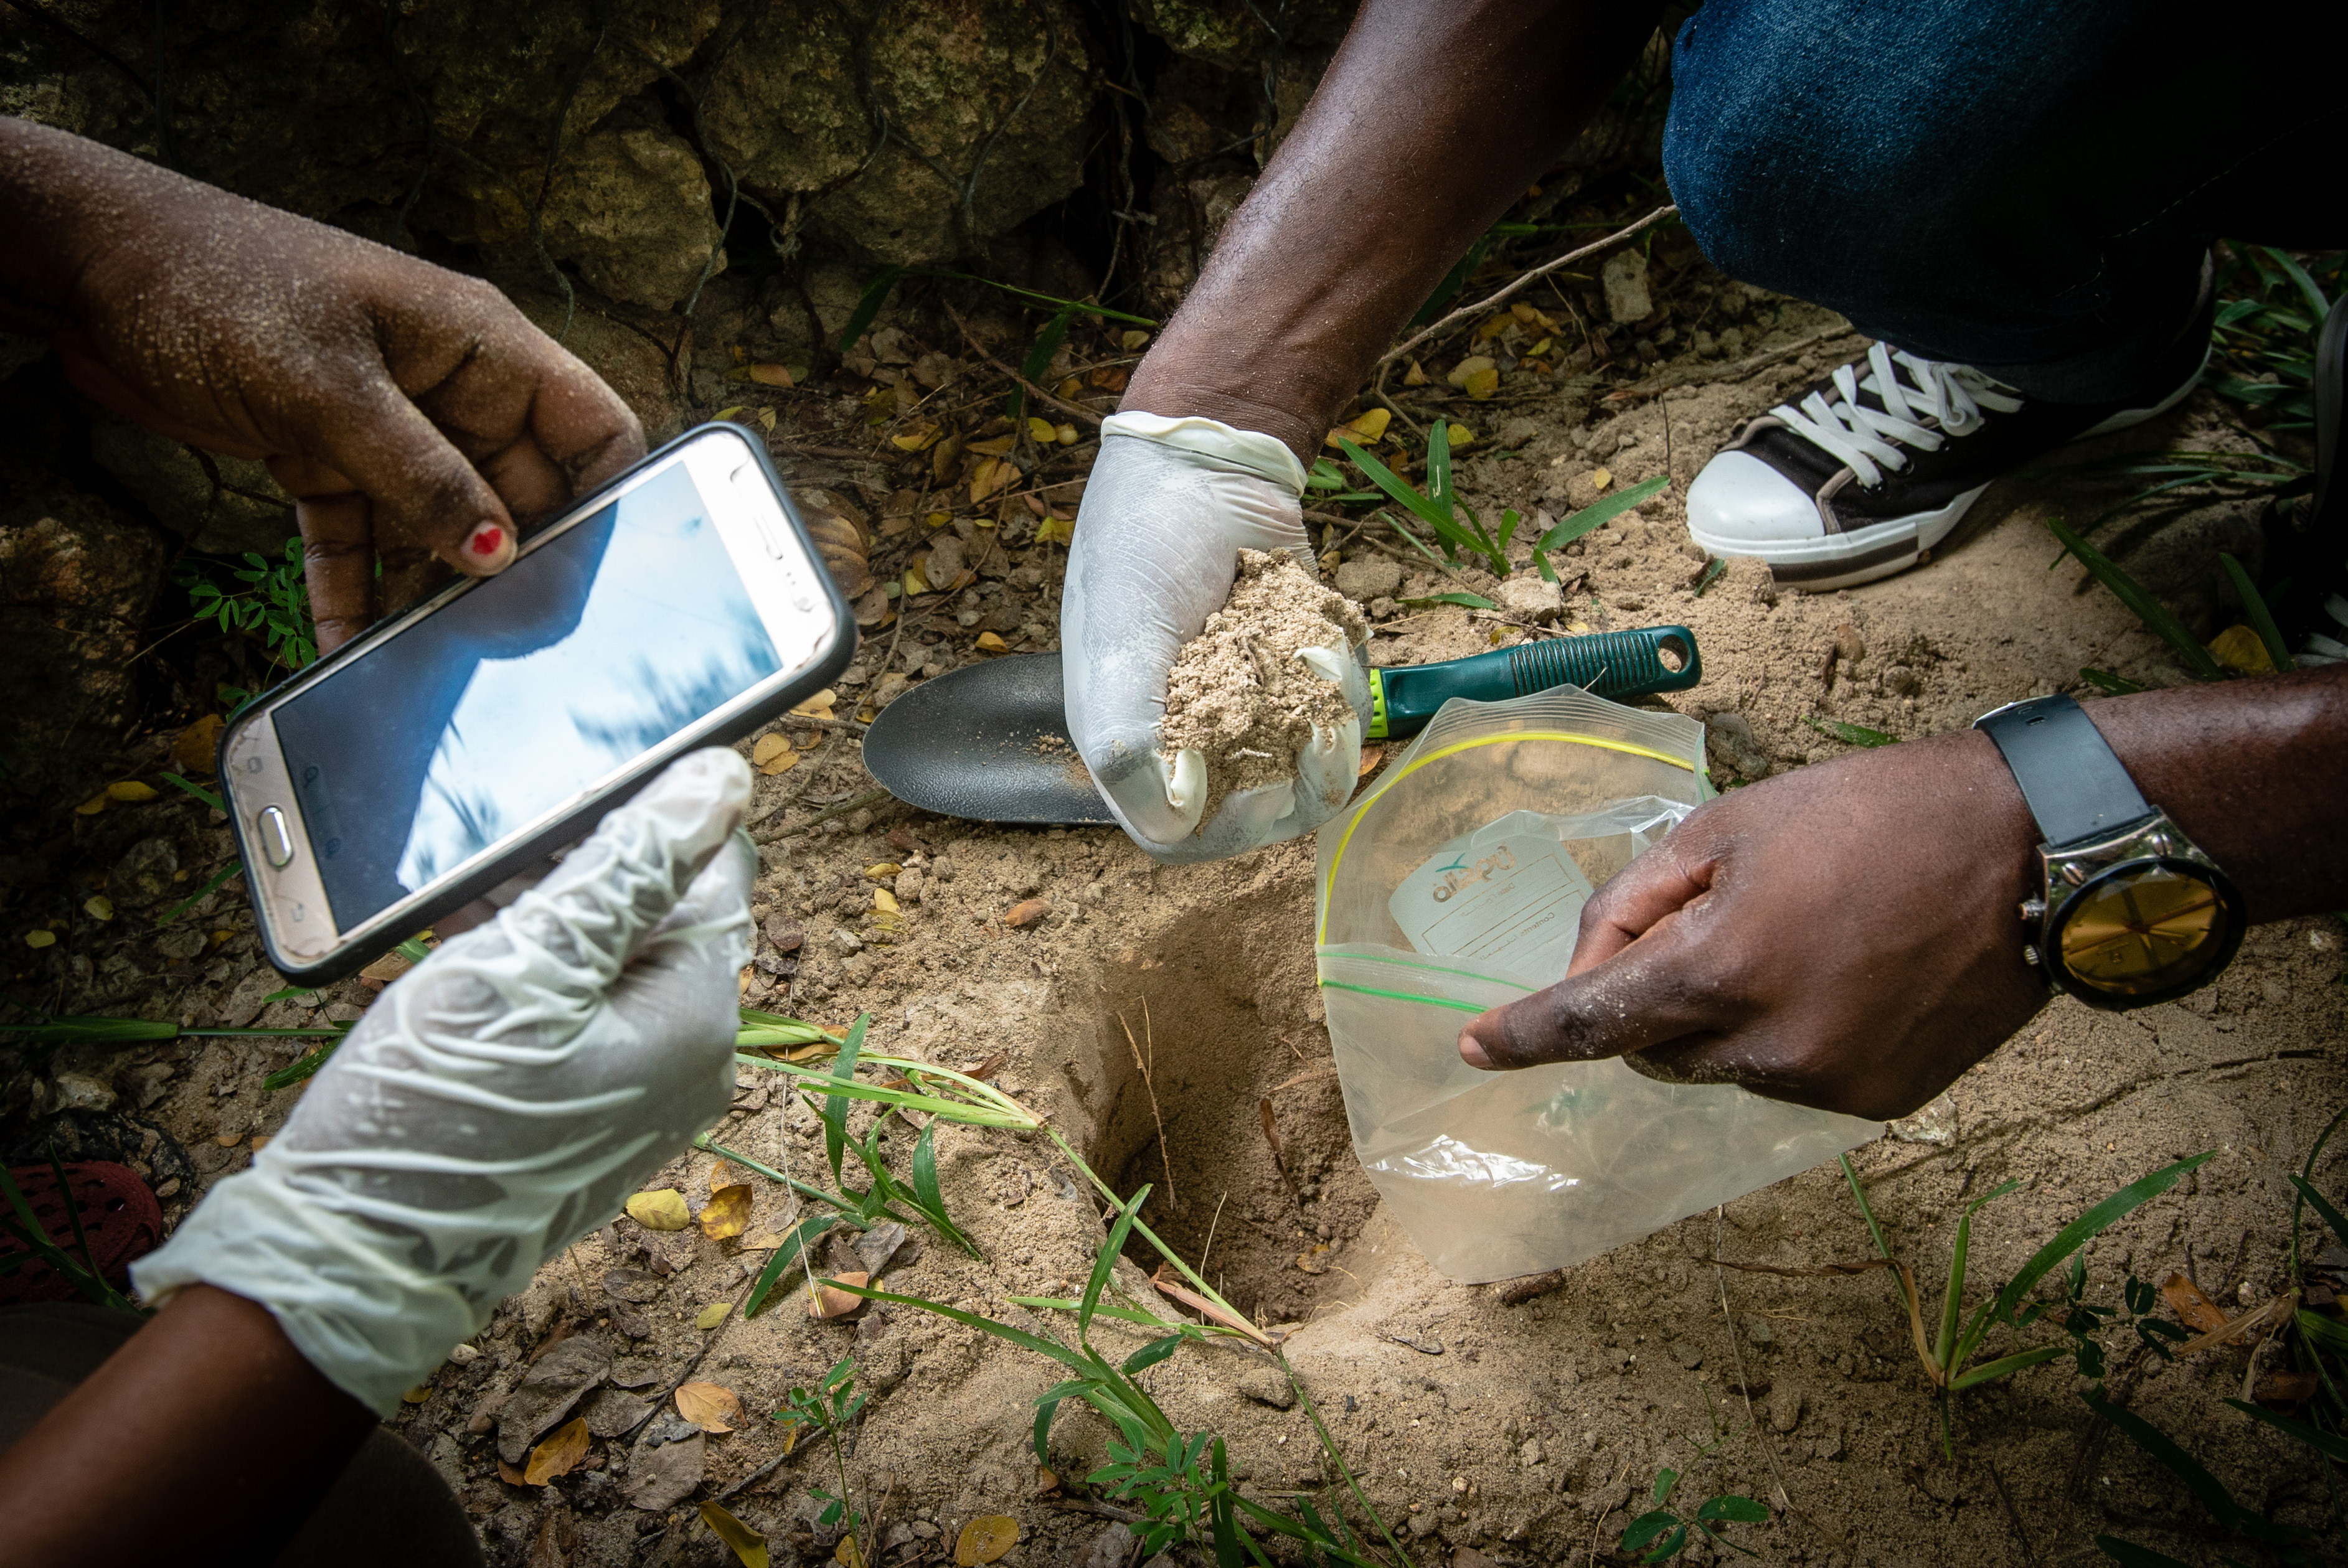
\includegraphics[width=\textwidth]{DSC05592.jpg}  

\subsubsection{Field Sampling Procedure}

Mappers used the following procedure as defined by JBA prior to commencement:
\begin{enumerate}
\item Navigate to the pre-defined sampling location.
\item Check the site is safe. If not, move on to the next site, and record the reason using ODK Collect.
\item If a sample cannot be taken (there may be a building or water body preventing access) the following procedure should be used: a suitable point within 500 metres of the defined sample location should be found by moving in a northerly direction. In some cases, points may simply not be accessible. In this case a reason should be recorded.
\item Once a suitable sample location has been identified use ODK Collect to record the relevant information by completing the survey form.
\item Use ODK Collect to take four photographs of the typical site surroundings (facing north, east, south, and west).
\item Begin taking the surface sediment sample using the following procedure:
\begin{enumerate}
\item Identify the area where you will take the sample. This should correspond
approximately to the sample point location, however it does not need to be exact.
\item Take a photograph of the ground before the sampling takes place
\item Remove the top layer of surface sediment using a pre-cleaned trowel or scoop (3 cm should be removed and discarded)
\item Collect one bag of sediment a depth between approximately 3cm - 7cm (TOP sample) and another from a depth approximately between 7cm and 15cm (BOTTOM sample). A tape measure should be used to measure the depths.
\item Place the collected sediment into plastic bags and tightly seal the them. If the bag appears at risk of breaking open the sample should be double bagged.
\item Each bag should be labelled with the unique site ID, either TOP or BOTTOM sample and the date using an indelible marker pen.
\item Move on to the next sample point.
\end{enumerate}
\end{enumerate}

\subsection{Laboratory Analysis}

The pair of samples---top and bottom---from each site was passed through a set of progressively finer-meshed sieves, resulting in nine separate fractions. Each fraction was weighed. The resulting measurements, which represent the proportion of each sediment particle size at each site, were recorded.

\subsubsection{Materials}
%\begin{wrapfigure}{r}{0.2\textwidth}
%  \centering
%  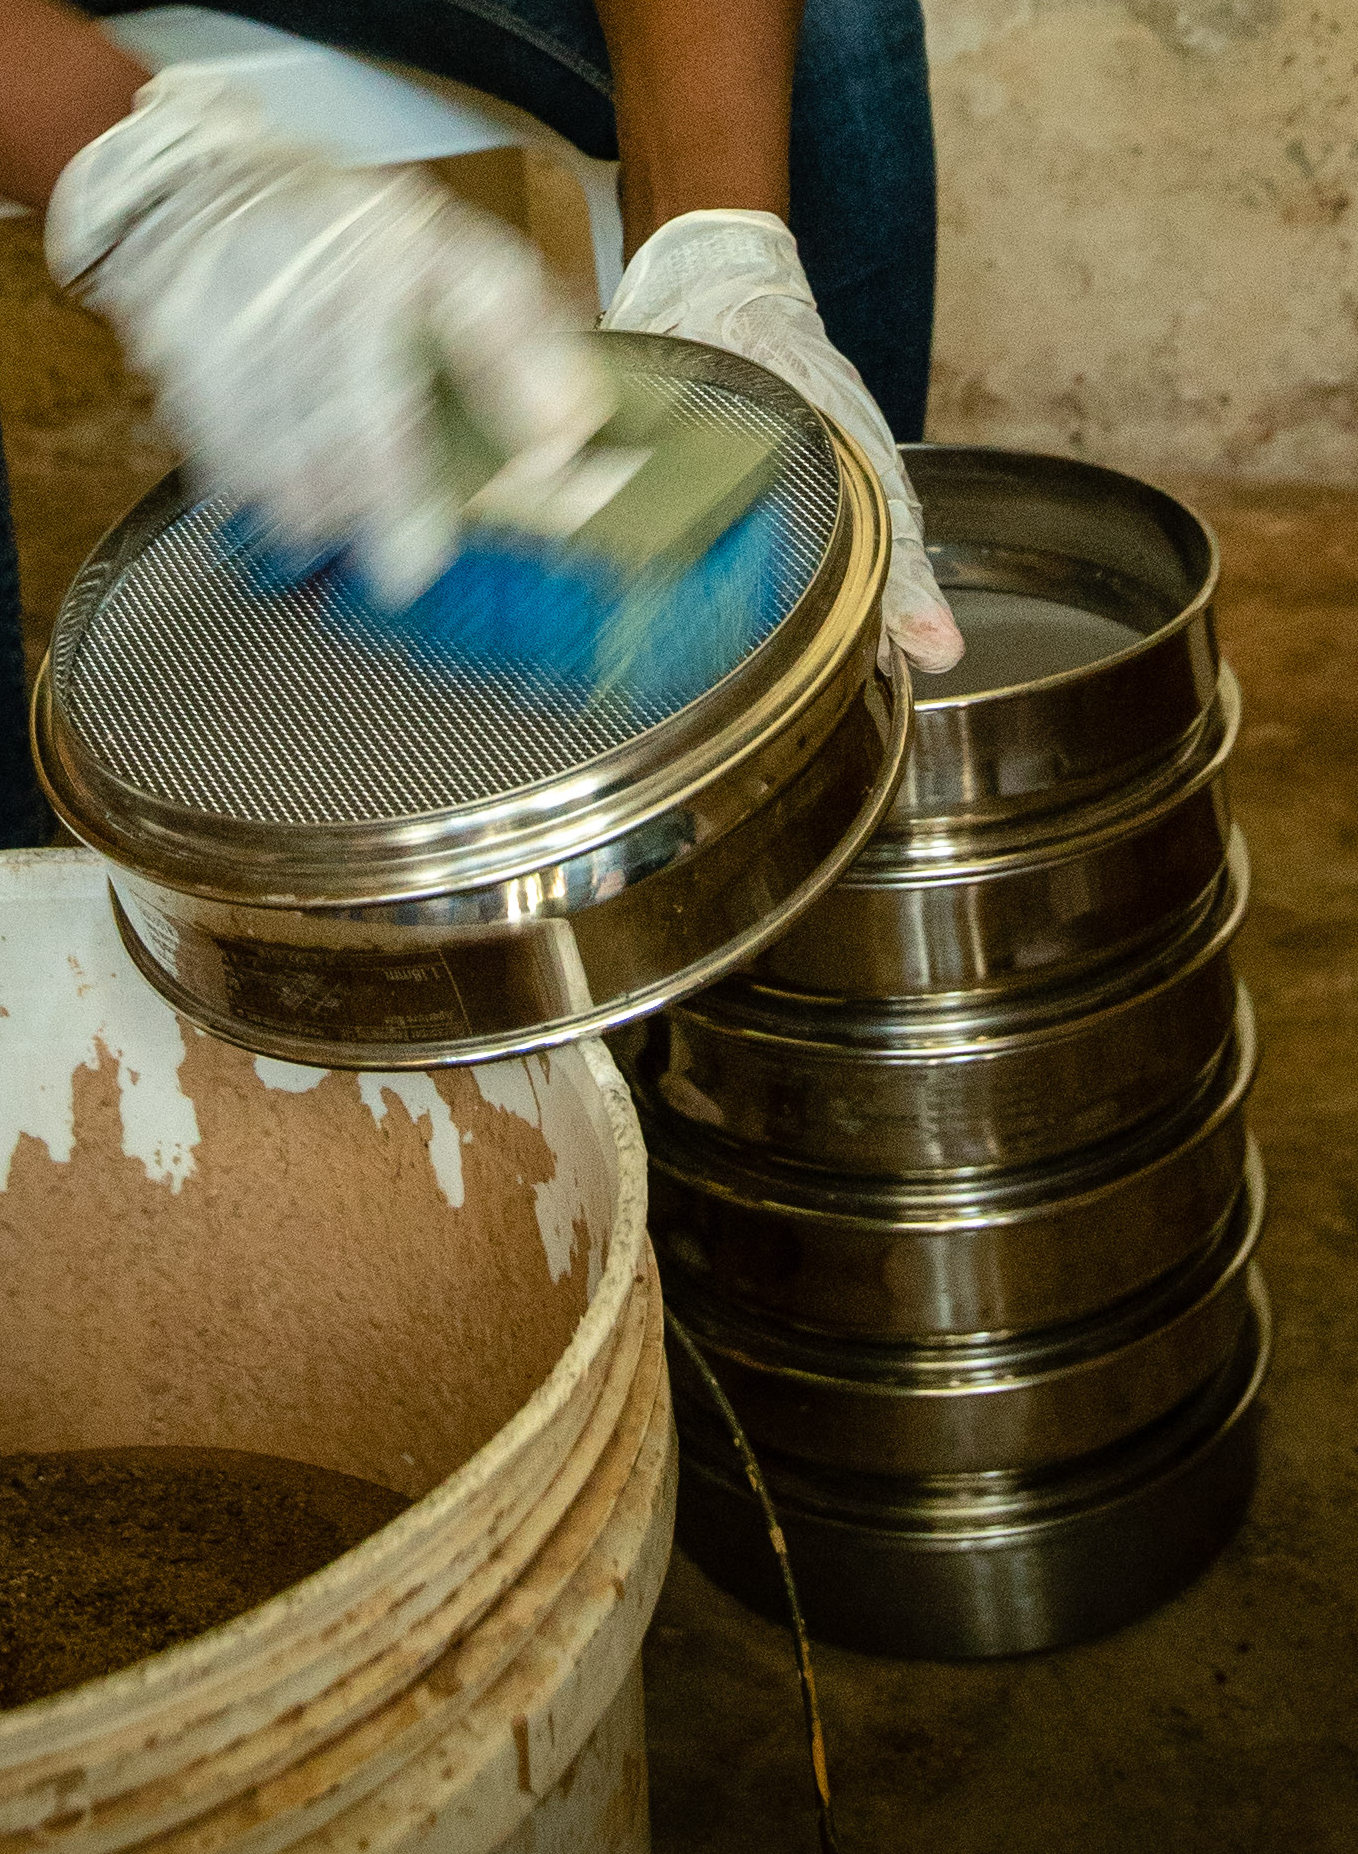
\includegraphics[width=0.18\textwidth]{DSC05543_cropped.jpg}
%\end{wrapfigure}
The following materials were used:

\begin{itemize}
  \item Set of metal sieves
  \item Scales
  \item Handwash station and gloves
  \item Brush, cloth, and towel for cleaning sieves
  \item Android phone with ODK Collect and sieving survey
\end{itemize}

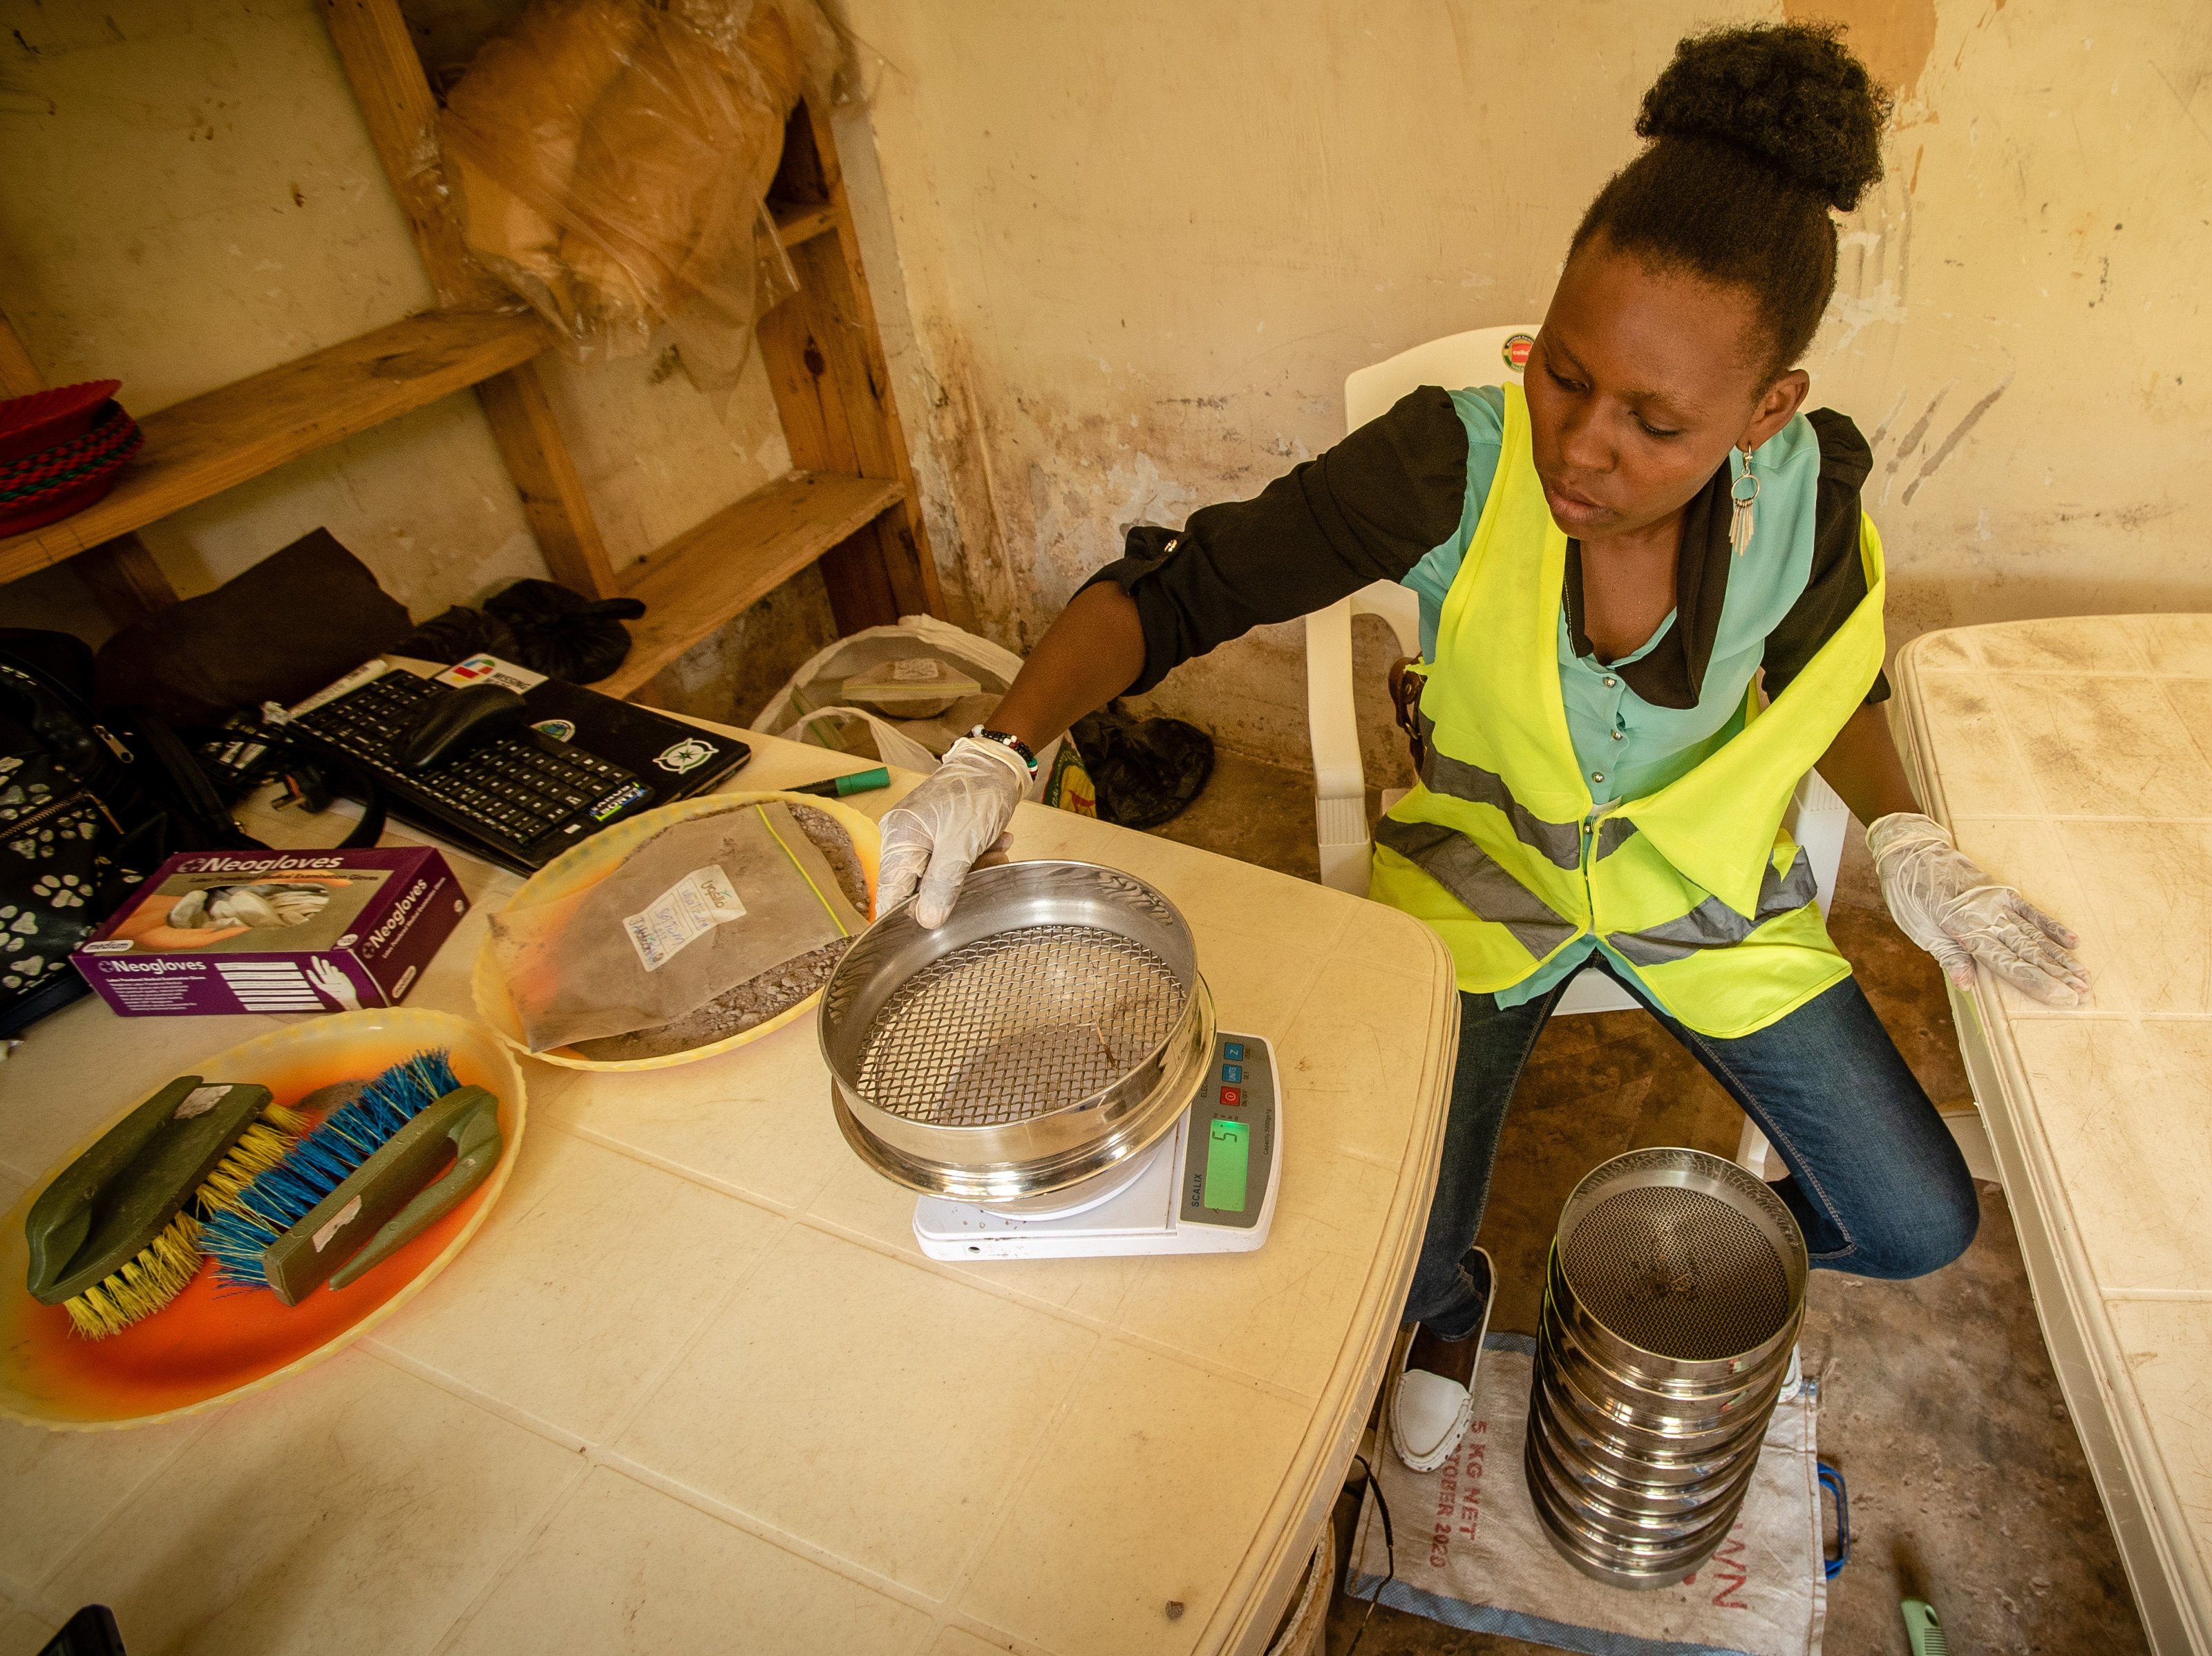
\includegraphics[ width=\textwidth]{DSC05570_cropped.jpg}

\subsubsection{Sieving and Data Entry}
The following procedure was used for the seiving:

\begin{enumerate}
  \item If samples are moist, they should be dried before analysis by being placed in the sun---though not exposed to wind---in a clean dry dish. 
  \item The following steps should be performed for both samples, beginning with the TOP sample.
  \item Weigh about 500g of sediment from the bag into a weighing dish.
  \item If sediment particles are lumped or conglomerated, crush the lumped particles until they become loose.
  \item Determine the mass (weight in grams) of each sample before sieving.
  \item Prepare a stack of sieves. Those with larger opening sizes are placed above the ones with smaller opening sizes. The lowest on the stack is a simple pan which retains the sediment that passes through the finest sieve.
  \item Make sure all sieves are clean---if any particles are stuck in the openings poke them out using the brush.
  \item Weigh all empty sieves and the pan separately. Record the results in ODK Collect.
  \item Pour the sediment into the stack of sieves from the top and place the cover on top. Shake the sieves carefully so the sediment filters through---this may need to be done for 3 to 5 minutes.
  \item Stop shaking and measure the mass of each sieve + retained sediment. Record the results in ODK Collect.
\end{enumerate}

Initially a Google Sheets spreadsheet was created to store the results. Each site (set of two samples) had a single tab on the spreadsheet, with the tab named for the site ID number. The sievers would use the move or copy sheet function in Google Sheets to create a new tab, rename that tab to the sample ID, and fill in the data. Calculations and checks were automatic. However, the RH team did not do well with this (see discussion in the \hyperlink{lessonslearned}{lessons learned} section). Therefore an ODK form was created to record the results, which eventually made for a more effective process. 

\newpage 
\section{Results and Analysis}
\label{resultsandanalysis}
The team sampled 643 sites, top and bottom (1286 soil sediment samples in total). The primary result is a table of masses representing the proportion of each size of sediment.

This data is primarily intended for use with erosion modeling. For users not equipped with erosion modeling skills and toolkits, and for sharing the results with the public, a visual map has been prepared that gives a good first impression of the characteristics.

\begin{figure}[h]
  \caption{The bars of the histogram---upper for the top samples and lower for the bottom samples---represent the proportion of each particle size.}
  \centering
  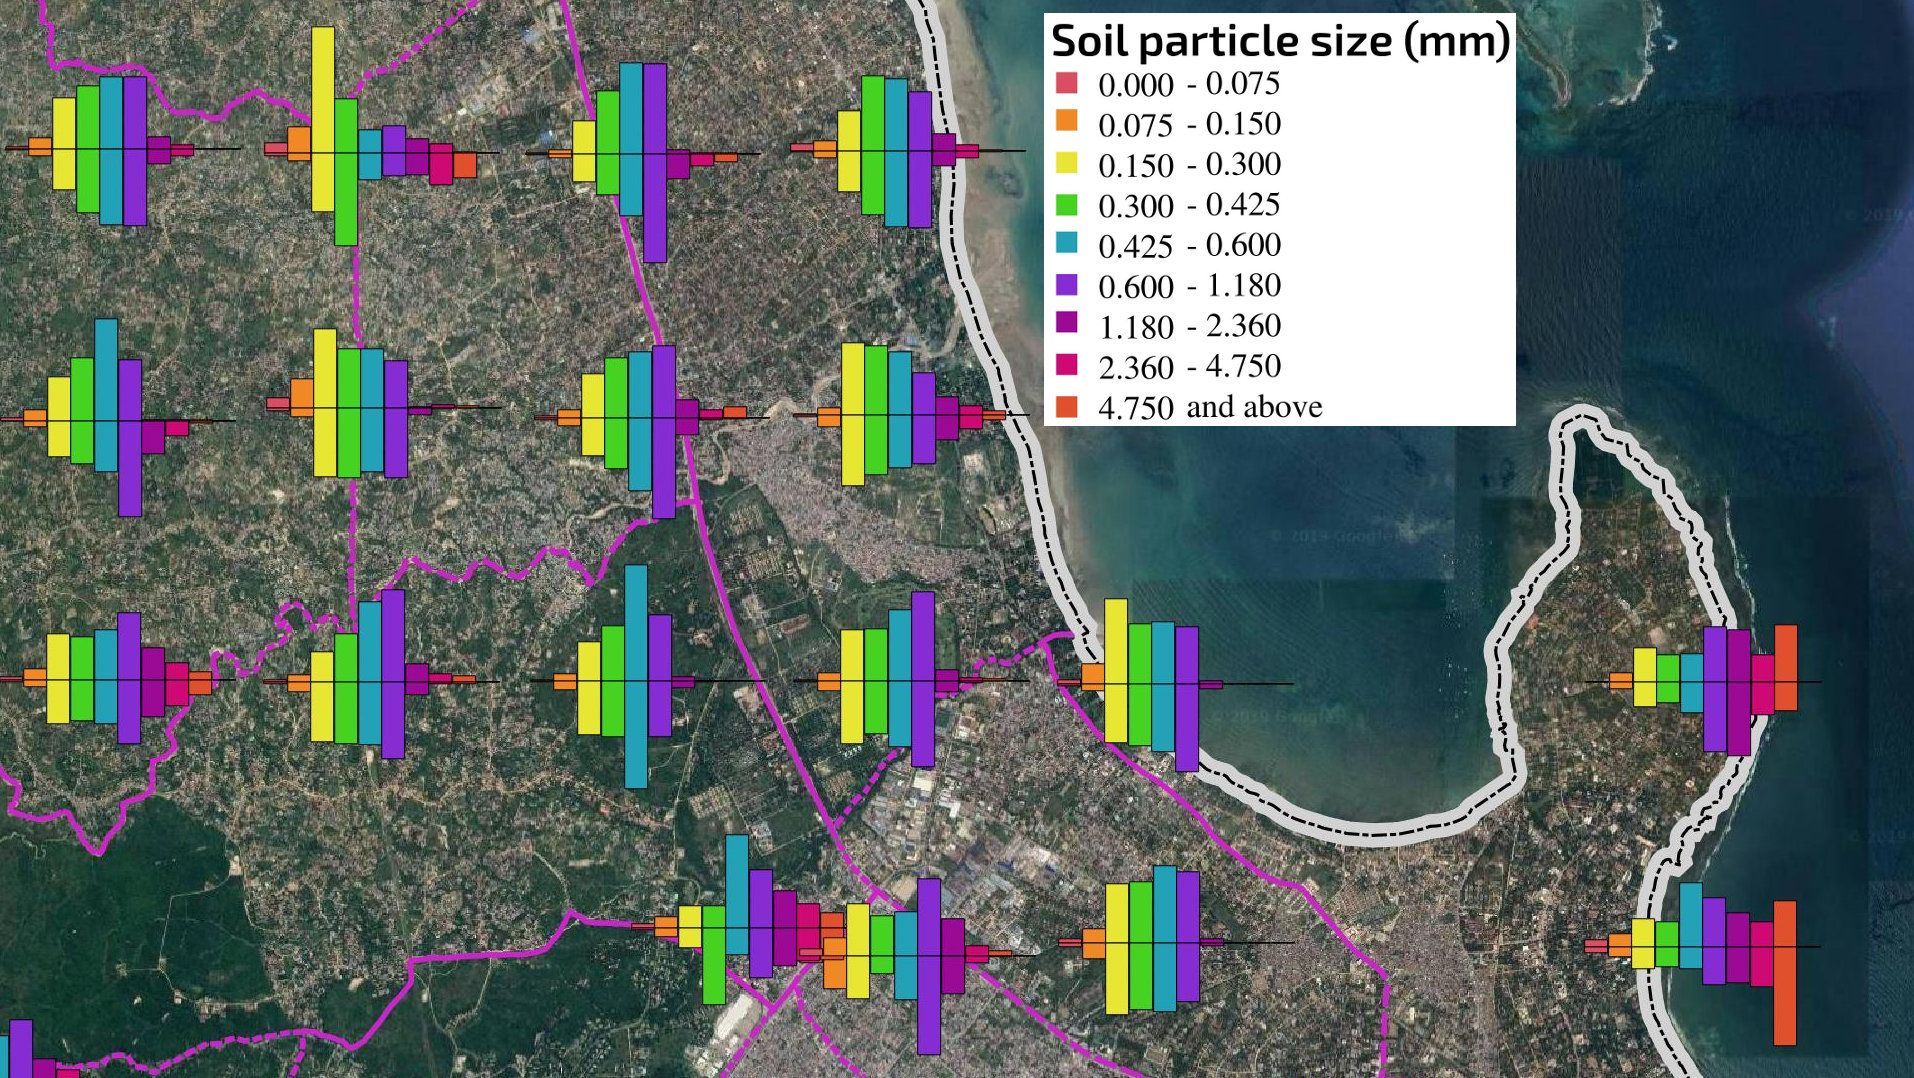
\includegraphics[width=1.1\textwidth]{soil_map_detail_peninsula_with_legend}
\end{figure}

The data has been uploaded to the \href{https://geonode.uhurulabs.org/layers/geonode\%3A_2019_02_26_dar_soil_sampling_final_results_v1}{UhuruLabs GeoNode}\footnote{\url {https://geonode.uhurulabs.org/layers/geonode\%3A_2019_02_26_dar_soil_sampling_final_results_v1}}. As open data, it is set to be downloadable by anyone, though only modifiable with permission.

An unfortunate limitation of the GeoNode platform is that it does not support the GeoPackage format for vector data, only the ESRI Shapefile format. Shapefiles have a 10-character limitation for column names, which results in truncation of some data headers. To mitigate, we have also uploaded the original CSV dataset which contains the full headers. 

The first use will be by JBA, who are entering the data into a model using the Revised Universal Soil Loss Equation (RUSLE) to better understand erosion as related to flood risk in Dar es Salaam.

\hypertarget{lessonslearned}{}
\section{Lessons Learned}
\label{lessonslearned}
The project generated a number of learning points that will be valuable for our team going forward, and that may be of use for others contemplating similar projects. In hopes that our lessons learned will facilitate others' efforts to make use of citizen science and community mapping methods for professional data creation and policy-making, we hereby present our experiences, both positive and negative.

\subsection{Field Data Collection}
\label{fielddatacollection}

\subsubsection{Budgeting time for seeking permissions}
A common challenge in this type of activity is seeking permission for doing what may be suspicious-looking activities (running around random areas of a major city with a shovel, for example). As the team put a fair bit of time and effort into this, no significant issues were encountered. However, it's important to budget time for this---it took several weeks to obtain permissions for all of the areas of Dar es Salaam that we visited, and this required staff time, transportation, etc.

\subsubsection{Inconsistent offset procedure}
Looking at the map of the sites that were actually collected, there were several for which it is not precisely clear what offset procedure was actually used when a given grid site was not accessible. While it is clear where the samples were actually collected---in all cases coordinates were taken for the actual site of colletcion---it's not necessarily clear how the team arrived at the offset location. In future, it would probably make sense to add more specific offsetting instructions, and add to the form a bit more structured explanation of what was actually done. Rather than just a comment field, a field in the survey form specifically asking for a description of the offset procedure used could be implemented.

\subsection{Sieving and Data Entry}

Several serious problems were encountered during the sieving and data entry procedure. Revisiting approximately seventy sites was required as a result of poor quality control. Critical issues included insufficient investment in the recording/data entry format, and insufficient quality control and feedback.

\subsubsection{Failure to realize the sensitivity of the error thresholds}
When looking at individual measurements anecdotally, we found that most were of high quality. In other words, it was possible to examine a few dozen measurements and only find one or two potential errors, which on the surface appeared to show that things were going well. This was grossly misleading!

In fact, 18 precise measurements (9 top and 9 bottom portions) are needed for a single site/sample to be correct, what looks like a low error rate upon a cursory inspection is actually quite a high one! A single weighing or data entry mistake over 10g in 100 measurements makes 20\% of the sites invalid; to get 99.45\% of sites within the acceptable threshold of 2\% discrepancy (not even that great an accomplishment) requires less than one in 400 measurements being out by more than 10g. 

This doesn't even take into account the 20-odd additional measurements per site, including the initial total masses of the top and bottom samples,and the empty sieve masses (these were much easier to get right as they are very consistent, but there were still a few errors in these measurements in the dataset prior to rework).

At the end of the first round of measurements, over seventy sites (more than 10\% of the total) had larger than 2\% discrepancies between the initial sample mass and the sum of the fractions, and were therefore invalid. In a few cases we were able to trace the specific error by comparing the two places the data were recorded (a Google Sheet and an ODK form), but we were forced to completely redo seventy sites.

We advise anyone doing similar projects to implement rigorous quantitative quality checks very early on. We certainly wish that we had done so. During our rework phase in February of 2019, we successfully migitated this by:

\begin{itemize}
  \item Simplyfying our data entry process (eliminating the Google Sheet data entry and using ODK Collect exclusively),
  \item Adding extra checks as calculations/notes in the ODK form to flag any discrepancies such as negative masses or discrepancies in sums immediately,
  \item Having a full-team meeting at the end of each analysis day with a supervisor--who was not part of the actual sieving team---to pull all of the data from the server and view it in a spreadsheet and map looking for discrepancies, and
  \item Retaining the sieved sediment until after the day's results were reviewed, as well as collecting larger samples in the field in order to have backup samples in case of loss/error.
\end{itemize}

  
\subsubsection{Field work outpacing analysis, insufficient early feedback}
As the team felt that the field work would be the most difficult part (and certainly it was the larger consumer of time and resources), we focused on it, and failed to become alarmed when the analysis (sieving) work fell behind. This contributed to there being a substantial backlog of sieving to be done at the end of the field collection, but also contributed to our not discovering the high proportion of discrepancies until long after the field work was complete. Had we been sieving as quickly as we'd been collecting, and creating interim compiled datasets from the outset, we'd have avoided most of the rework.

\subsubsection{Inadequate backup of samples}
We did not build backup into our analysis; we discarded all of the sediment immediately after sieving and measurement, and only collected enough for a single round of sieving at each site. During the rework phase in February of 2019, we built in two redundancies:

\begin{itemize}
  \item We collected 1kg of sediment for each sample (2kg including top and bottom) in order to have enough left for re-analysis if anything went wrong, and
  \item We did not discard the sediment after sieving until both samples for the entire site were confirmed correct at the end of each day with a project supervisor.
\end{itemize}

We heartily recommend both measures to anyone contemplating a similar project.

\subsubsection{Data entry system design}
It's critical to design the tools carefully. We encountered problems in data entry, in part because we didn't invest enough in making sure the system was robust and simple.

We began using a Google Sheet template. This template contained data entry cells for the team to enter measurements, and formulas to calculate results such as sediment retained (mass of sieve + sediment - mass of empty sieve). Conditional formatting was used to highlight errors such as negative masses (indicating measurement problems) or discrepancies above 2\% between the initial mass of a given sample and the sum of its fractions. We expected the teams to duplicate a template tab in the spreadsheet for each sample site, resulting in a spreadsheet with hundreds of tabs full of data that would later be consolidated. This was problematic for a number of reasons.

\begin{itemize}
  \item The formulas and conditional formatting were difficult to protect from accidental modification.
  \item The latency of Google Sheets in a low-connectivity environment sometimes caused slow updates, resulting in mistakes.
  \item The method of duplicating tabs created a dataset that was extremely difficult to look at in a consolidated fashion. Google Sheets (and other spreadsheet programs such as Microsoft Excel or Libreoffice) do not have good facilities for ordering sheets, making searches for particular tabs and finding duplicates very difficult.
  \item Google Sheets, like most spreadsheet platforms, has a limit on the number of tabs that can be created in a single document (in the case of Google Sheets as of this writing, the limit is 200 tabs per document). This necessitated the creation of multiple workbooks/documents, which further complicated the task of sorting, searching, and de-duplicating.
  \item Google Sheets are vulnerable to multiple editor errors. More than one person can access a sheet simultaneously, and it's relatively easy to find oneself in the wrong sheet, or to make a mistaken edit with an unintentional keystroke. Even more terrifying is the possibility of data deletion, which---again in contrast to a submission-based system such as Google Forms or ODK---can be done accidentally. 
\end{itemize}

We considered several options for this. The Google Forms platform allows for the entry of multiple data points which aggregate to a single spreadsheet. This would probably have been a better option. However, since the team was already familiar with OpenDataKit from field work, and the ODK facilities for implementing real-time calculations and error warnings are quite robust, we chose to use ODK.

We made the decision to continue using both the Google Sheet as well as ODK. This, in retrospect, was probably a mistake. Using both platforms simultaneously simply resulted in more errors accumulating---we would almost certainly have been better off using only one method and being rigorously consistent with it. The team tended to enter into one platform and then copy into the other, which simplycreated more data entry errors.

During our rework phase, we used only the ODK platform. We ensured data backups by performing daily end-of-day data downloads---which also served as quality control points---and stored the results on local devices. This worked very well, and we recommend this procedure (and will ourselves use it in the future).

Another possibility, if data entry on a computer rather than mobile device is preferred, would be to use a desktop database management package, which allows the creation of data entry forms.

\subsubsection{Miscellaneous points for improvement}
\begin{itemize}
  \item The samples were supposed to be shaken in the sieves for three minutes. This was initially done without a stopwatch, which upon observation resulted in quite a lot of variation in the shaking time (sometimes more and sometimes less than the requisite three minutes). We corrected this after a few days, but we can't be certain that this did not affect the quality of a few early samples (though it seems unlikely as the sediment fractions were all visually quite well separated).
  \item The samples were initially being dried on styrofoam boards or plastic tarps. This left residue on the drying area, which tends to be fine particles that are lost to the measurements. Furthermore, the process of transferring the sediment from the bags to the drying area and back seems to result in a small amount of winnowing (dust flying off as the transfers took place). The team procured some plastic trays for drying so that each sample could be transferred without winnowing loss or leaving fines behind.
\end{itemize}

\end{document}